\documentclass{article}
% Change "article" to "report" to get rid of page number on title page
\usepackage{amsmath,amsfonts,amsthm,amssymb}
\usepackage{setspace}
\usepackage{Tabbing}
\usepackage{fancyhdr}
\usepackage{lastpage}
\usepackage{extramarks}
\usepackage{url}
\usepackage{chngpage}
\usepackage{longtable}
\usepackage{soul,color}
\usepackage{graphicx,float,wrapfig}
\usepackage{enumitem}
\usepackage{morefloats}
\usepackage{multirow}
\usepackage{multicol}
\usepackage{indentfirst}
\usepackage{lscape}
\usepackage{pdflscape}
\usepackage{natbib}
\usepackage[toc,page]{appendix}
\providecommand{\e}[1]{\ensuremath{\times 10^{#1} \times}}

% In case you need to adjust margins:
\topmargin=-0.45in      % used for overleaf
%\topmargin=0.25in      % used for mac
\evensidemargin=0in     %
\oddsidemargin=0in      %
\textwidth=6.5in        %
%\textheight=9.75in       % used for mac
\textheight=9.25in       % used for overleaf
\headsep=0.25in         %

% Homework Specific Information
\newcommand{\hmwkTitle}{Progress Report 2}
\newcommand{\hmwkDueDate}{Monday,\ November\  5,\ 2018}
\newcommand{\hmwkClass}{Final Project}
\newcommand{\hmwkClassTime}{CSE 597}
\newcommand{\hmwkAuthorName}{Yueze Tan}
\newcommand{\hmwkNames}{yut75}

% Setup the header and footer
\pagestyle{fancy}
\lhead{\hmwkNames}
\rhead{\hmwkClassTime: \hmwkTitle} 
\cfoot{Page\ \thepage\ of\ \pageref{LastPage}}
\renewcommand\headrulewidth{0.4pt}
\renewcommand\footrulewidth{0.4pt}

%%%%%%%%%%%%%%%%%%%%%%%%%%%%%%%%%%%%%%%%%%%%%%%%%%%%%%%%%%%%%
% Make title

\title{\vspace{2in}\textmd{\textbf{\hmwkClass:\ \hmwkTitle}} \\
\vspace{0.1in}\large{ \hmwkClassTime}\vspace{3in}}

\author{\textbf{\hmwkAuthorName} \\ \vspace{0.1in}
\hmwkDueDate }
\date{} % to take away today's date

%%%%%%%%%%%%%%%%%%%%%%%%%%%%%%%%%%%%%%%%%%%%%%%%%%%%%%%%%%%%%

\begin{document}
\begin{spacing}{1.1}
\maketitle

\newpage
\section*{Abstract}

In this progress report, we discuss about the Jacobi solver for Poisson equation with Debye-Huckel's shielding term, along with its parallelization using MPI. The justification of the parallelization method and the profiling of the code are also discussed in this report, after which we show the scaling results for multi-core calculations.

\section{Problem of Interest}

The problem is related with solving the electrostatic equation (Poisson equation) in a system with free moving charges and shielding effects, typical examples of which would be plasma or electrolytes. From Boltzmann's distribution we can obtain the equation describing the shielded, or compensated field:
\[(\nabla^2 - \lambda_D^{-2})\Phi=-\frac{\rho}{\varepsilon},\]
in which $\Phi$ is the electric potential, $\rho$ is the charge density which is contributed by other effects than shielding, like charge density induced by inhomogeneous distribution of polarization in a dielectric matter, and $\varepsilon$ is permittivity of the system. $\lambda_D$ is known as Debye length, which is a term coming from Debye-Huckel's linearization of the electric shielding effect.

For free-moving charge is common in various physical systems, charge compensation and spontaneous shielding effect could be widely observed in different kinds of condensed systems. In order to get a more accurate solution in these systems, solving the electrostatic equation with Debye length term is a necessary step. The distribution of electric potential is an interested topic in various fields, like materials science, condensed matter physics and chemical engineering, where electrolytes are extensively discussed.

Other numerical methods could also be applied to solve this problem, as what could be done for many other different types of PDEs. One possible way is using finite-element method (FEM), in which we discretize the system into piecewise functions, and then transform the problem into a integration form:
\[\int_V\left[(\nabla^2-\lambda_D^{-2})\Phi+\frac{\rho}{\varepsilon}\right]v_i\;\mathrm{d}V=0,\]
in which $v_i$ is a set of specially chosen functions to simplify the integrations.

Or we can use fast Fourier transform (FFT) to solve this problem, by transforming the original field into Fourier spectrum and then solve the algebraic equation in the frequency domain:
\[(k_1^2+k_2^2+k_3^3-\lambda_D^{-2})\Phi^K=-\frac{\rho^K}{\varepsilon},\]
and by taking inverse FFT (IFFT) on the spectrum we can get the field in real space. Such a method has already been used to solve the conventional electrostatic problem in phase-field models, see \citep{li2002}.

It might be of the readers' interest that this problem has an analytical solution, which is based on its Green function:
\[ \Phi(\mathbf{r}) =
\int _V \frac{\rho(\mathbf{r'}) (\mathbf{r} - \mathbf{r'}) \exp(|\mathbf{r} - \mathbf{r'}| / \lambda_D)}{|\mathbf{r} - \mathbf{r'}|^3} \;\mathrm{d}^3 \mathbf{r'} +
\oint _{\partial V} \frac{\sigma(\mathbf{r'}) (\mathbf{r} - \mathbf{r'}) \exp(|\mathbf{r} - \mathbf{r'}| / \lambda_D)}{|\mathbf{r} - \mathbf{r'}|^3} \;\mathrm{d} S.\]
Basically, this solution is a modified version of the regular electrostatic solution for Poisson equation, but equipped with an exponentially decaying factor so the electric potential drops much faster, which is what we are expecting from a shielding effect.

However, carrying out such an integration is practically unfavourable for most cases, as the time consumption is not satisfying, and precision of numerical solution is also suspicious since the expression to be integrated is divergent at $\mathbf{r} = \mathbf{r'}$. Besides, for most cases the boundary condition is of Dirichlet's type, which means $\sigma(\mathbf{r'})$ is unknown on the boundary of the integrated region. Therefore, a numerical way of solving the original PDE is practically more favourable.


\section{Parallelization}

To solve this problem, we use Jacobi's iterative method. The electric potential field is smashed into a vector, and the operator is changed into its matrix form, which could be written as
\[\mathbf{A\Phi}=\frac{\mathbf{\rho}}{\varepsilon}\]
The major time consumption is expected to take place during this iterative solver itself.

The parallelization method used in this project is MPI. Since the system matrix $\mathbf{A}$ could become considerably large for those product-size problems, it is a better practice to use a distributed memory method to carry out the parallelization. Also, such a method enables the possibility of running the program on distributed nodes, which means it could be executed with more computational resource and easier to scale compared to those shared memory methods.

As Jacobi iterative solver needs communications during solving to update the target vector on each process, Map-reduce is not an appropriate method for this problem. OpenMP and Threads are both shared-memory methods and are less favoured as discussed above. The iterative method could be decomposed to row-wise operations for the matrix, and during the calculation step (after which will be the updating of vector), there is no need to get access to other matrix elements located on other processes, while \texttt{MPI\_Broadcast()} is enough to take on the task of updating of the vectors, therefore there is no need to make use of global address space, which means there is no need to use PGAS method.

MPI method requires a drastic reconstruction of the original code, therefore nearly every class needs rewriting. However, the most important parallelizations are on the initialization of A matrix and the iterative solving steps. Since each process only stores part of A matrix, this could be generated in a parallel way for this program. During the iterative solving of the linear equation, we need to multiply the vector by the matrix to get the updated value, while this could be done independently for each row of vector, therefore by storing the matrix distributively, the matrix multiplication could also be parallelized, which is the most significant part of the parallelization for this certain method.

As most of the time consumption for solving takes place in Jacobi solver itself, it is possible that the percentage of parallelization is very close to 100\%, at least higher than 95\%, at first glance. However, from the following discussion on profiling of the parallel version of the code, we will find that parallelization is not a free lunch with the cost of communications between processes, especially broadcasting of data, whose time consumption can even grow as the parallelization size gets larger. A small portion of the code, such as I/O operations, are intrinsically not able to be parallelized. Besides, broadcasting the right hand side of the linear equation to every process during the initialization is also a step which could not be parallelized, though all these vector operations are typically must faster than matrix operations. For a linear system with size of $N$, this will cost around $1/N$ of total running time.

Setting up the matrix is similar to that of sequential version of program, except that now only a piece of matrix is stored on one single process, and each process only needs to generate a part of it, therefore as could be seen in the source code, in the generation of system matrix, we add conditions to jump through the loops, so that only a small portion of elements will be covered on each process. Generation of b vector (right hand side) is similar, but as this vector is stored with a complete copy on each process, we need to use broadcast after the generation. These are the obvious differences in generation of the matrix and the RHS vector.

\section{Profiling}

\subsection{Serial}

The profiling is done with a $ 20\times 20 \times 20$ grid number of 3D-field, with Dirichlet's boundary condition, therefore dimension of the linear system is 5832. The profile result for the serial code is shown as below:

\begin{figure}[H]
  \centering
  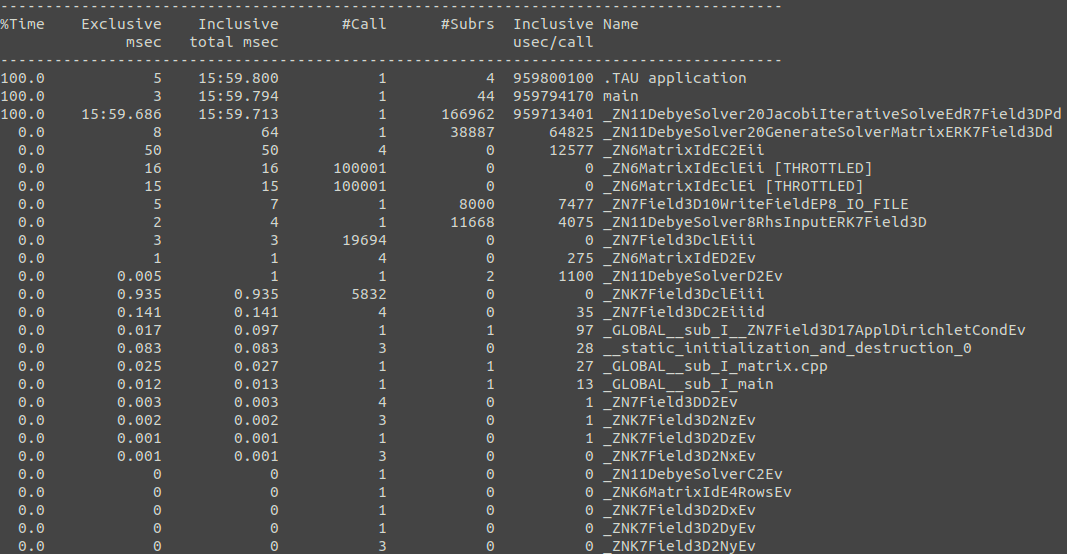
\includegraphics[width=\linewidth]{output/serial-previous-text.png}
  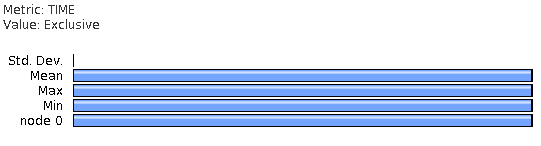
\includegraphics[width=0.6\linewidth]{output/serial-previous.png}
  \caption{The profile results of serial code.}
  \label{fig-testcase}
\end{figure}

As could be seen, nearly 100\% of time is consumed on the \texttt{JacobiIterativeSolve()} function, which is the major function of iterative solver itself. This is just the same as our expectation discussed previously.

As nearly all time consumption comes from the solving of equation itself, there is no obvious and simple way to upgrade the efficiency. Here we are simply changing the compiler's flag from \texttt{-O2} to \texttt{-O3}. Other possible ways might include changing the compilers, rewriting the code to make full use of CPU cache, or try to optimize the algebraic operations to make full use of FMA.

Below is the updated profile with the new optimization flag.

\begin{figure}[H]
  \centering
  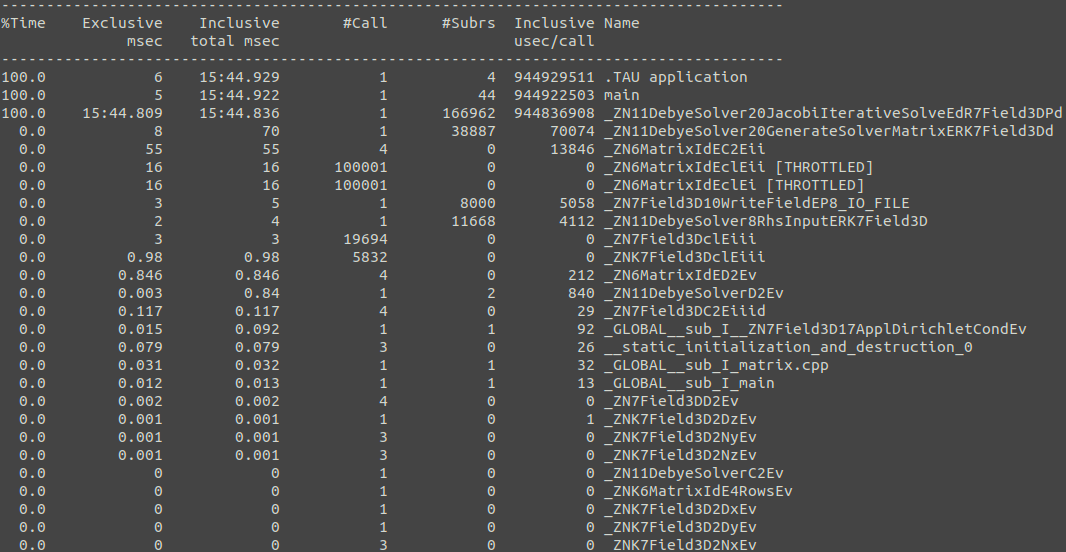
\includegraphics[width=\linewidth]{output/serial-improved-text.png}
  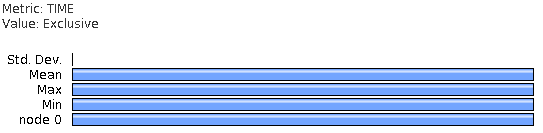
\includegraphics[width=0.6\linewidth]{output/serial-improved.png}
  \caption{The profile results of serial code with improved compiling flag.}
  \label{fig-testcase}
\end{figure}

As could be seen from the results, there is a slight improvement in the speed. For the same problem size, the time consumed decreases from 15 min 59 s to 15 min 45 s, shortened by around 1.5\%. However, this might also be influenced by other factors such as the load of server.

\subsection{Parallel}

The profiling is done with a $ 20\times 20 \times 20$ grid number of 3D-field (i.e., still sample size), with Dirichlet's boundary condition, therefore dimension of the linear system is 5832. The profile result for the MPI parallel version of code is shown as below, with \texttt{-np=10}:

\begin{figure}[H]
  \centering
  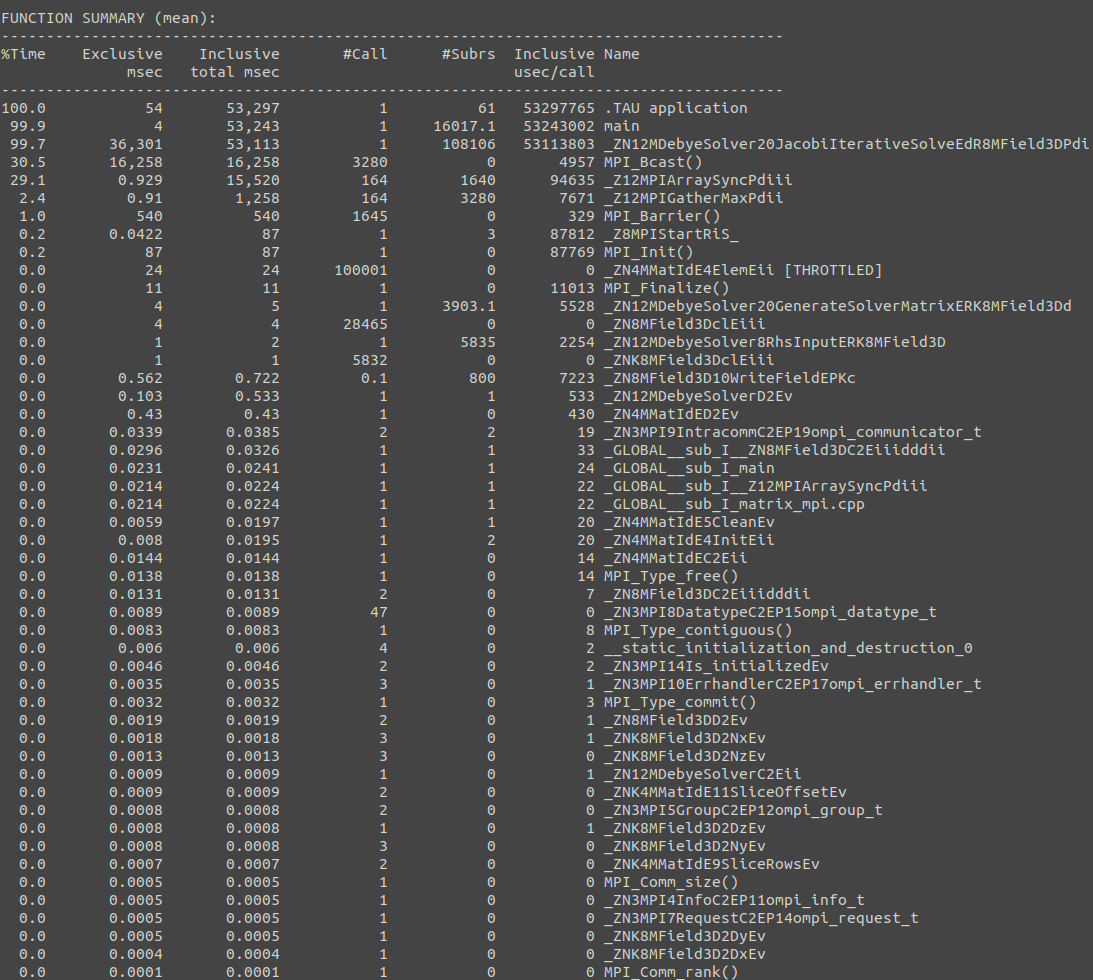
\includegraphics[width=\linewidth]{output/mpi-previous-text.png}
  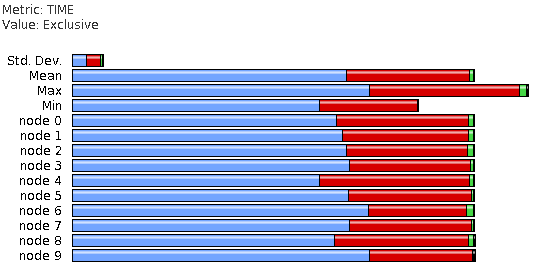
\includegraphics[width=0.6\linewidth]{output/mpi-previous.png}
  \caption{The profile results of parallel code.}
  \label{fig-testcase}
\end{figure}

As shown in the profile, the major contribution of the time consumption still comes from the algebraic operations inside of the solver itself (shown in blue). However, this time we see a significant contribution from the talk between processes, i.e., time consumption on \texttt{MPI\_Bcast()} (shown in red).

These two factors are both as expected, however, the time consumption on the talking is much higher than the initial guess, since it is obviously not at a scale of $1/N$. This might be related with specific computer architecture, or number of nodes involved (though we are only using one node here).

A direct comparison of speed could not be provided by the executable file with the profiling tool implemented, since the profile can induce noticeable difference between serial and parallel code. Here we only compare the execution time ratio of different functions for serial and parallel codes. As could be seen, the \texttt{JacobiIterativeSolve()} method is still the most time-consuming part, while at this case it is distributed onto different nodes, and the total amount of time is therefore decreasing, as expected.

Compared with the serial code in PR \#1, the parallel version of code is running with way much shorter time (the serial part of code is taken from the code in PR \#1), which could be seen from the profile results. However, the memory cost is slightly rising, since each node is now holding a complete copy of the RHS vector and solution vector. But this is not an obvious cost, since the size of matrix is thousands of times larger, while that is stored piecewise and shall not induce a strong memory increase.

As MPI communication is time-consuming for parallel code with \texttt{-np=10}, it is possible to substitute \texttt{MPI\_Bcast()} by other functions as \texttt{MPI\_Allgatherv()}, to see which has a higher efficiency. With such a modification, the profile is shown as below:

\begin{figure}[H]
  \centering
  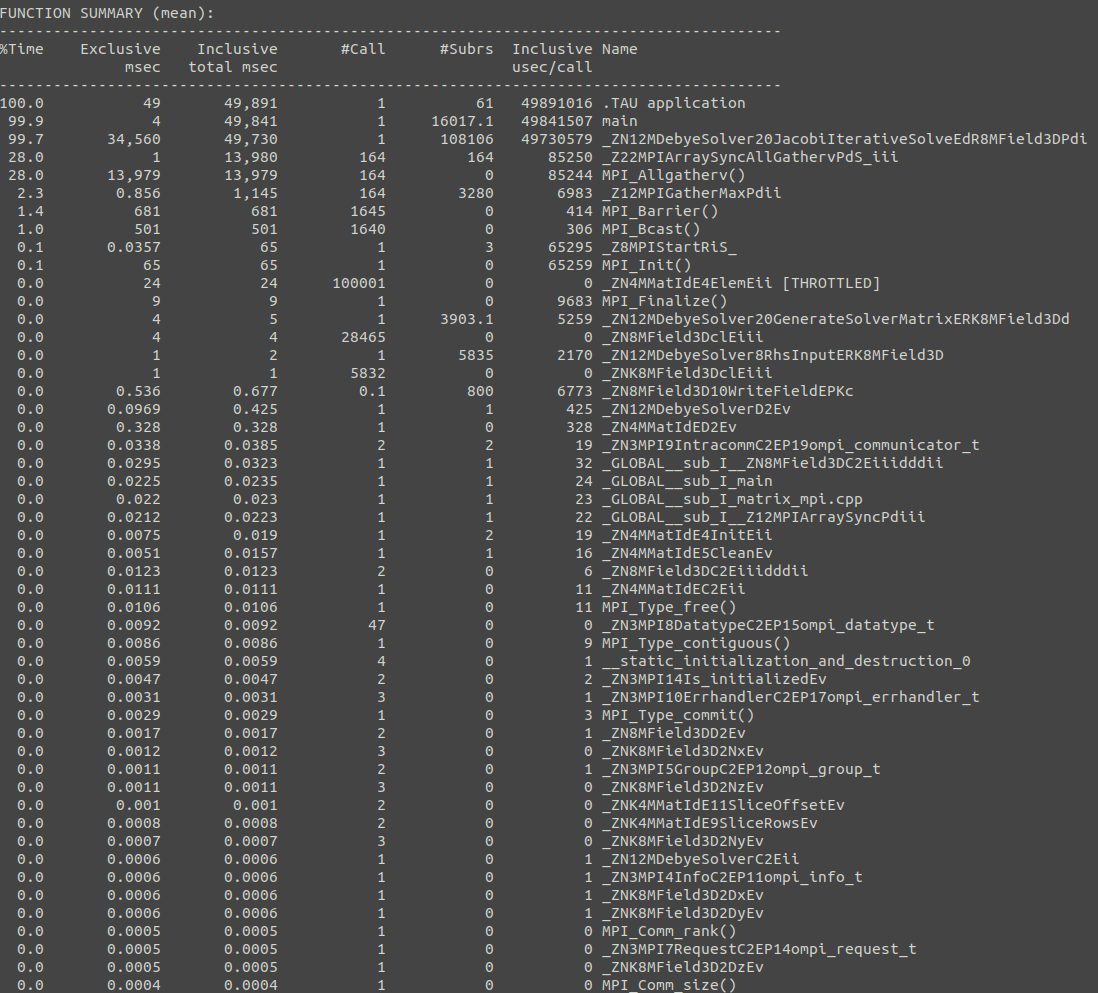
\includegraphics[width=\linewidth]{output/mpi-gather-text.png}
  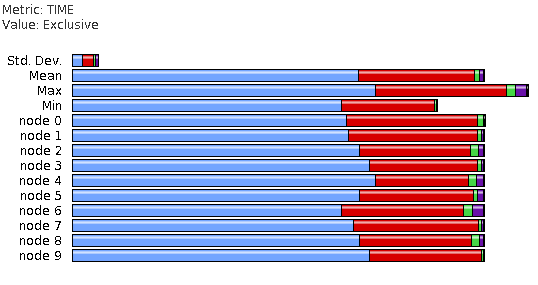
\includegraphics[width=0.6\linewidth]{output/mpi-gather.png}
  \caption{The profile results of parallel code with MPI\_Allgatherv().}
  \label{fig-testcase}
\end{figure}

After changing the MPI communication function, there is a slight accelaration in the average running time of the functions. Another way is to reduce the number of processes to no larger than number of cores on the node, see the scaling discussion below for details.

\section{Scaling}

\subsection{Strong Scaling}

The plot for execution time of strong scaling on login node of ACI is shown as below:

\begin{figure}[H]
  \centering
  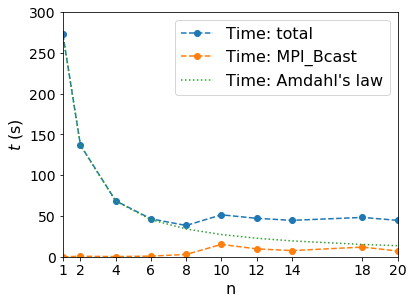
\includegraphics[width=0.5\linewidth]{output/scaling.png}
  \caption{The profile results of parallel code with MPI\_Allgatherv().}
  \label{fig-testcase}
\end{figure}

The plot starts with $N=1$, which is actually serial, with the same problem size as above examples. This size is already large enough to profile the speed up of parallelization, and starting from $N=1$ makes it easy to get the expected computation time from Amdahl's law. From this plot we could also see that the number \texttt{-np=10} is actually not a good choice for the parallel code profiling example, since it gives a large overhead of communication time between processes. However, this does not influence the validity of those discussions.

From the plot, it could be seen that \texttt{-np=8} should be used for speed for the sample-sized problem, while the best efficiency is reached at \texttt{-np=1}, where no communication happens. For a research problem, more processes with an acceptable efficiency will be preferred as this might be related with the cost of computational resources, therefore \texttt{-np=8} can be used as a result of balancing between performance and efficiency, if efficiency does not vary as the size of problem grows, which needs to be further investigated by weak scaling tests. Also, the communication cost rises drastically after $N \geq 10$, which can be related with the server and node structure, and could be varying on different architectures. For this test, since the login node has 8 cores, which could be confirmed with "\texttt{cat /proc/cpuinfo}", the speed up will be limited after that number, i.e., $N > 8$. Therefore, for nodes with more cores, using more processes, such as $N=10$, might be a better choice.

If we take $p \approx 100\%$ from the profile of serial code, then Amdahl's law could be written as

\[S=\frac{t_\mathrm{serial}}{t_\mathrm{parallel}} \approx s = \max{(N_\mathrm{processes}, N_\mathrm{cores})}.\]

However, this is only possible if no communication cost, which could even arise (seen from above), is considered. 

From the plot above, we can see that for $N \leq 8$, the speed is very close to ideal, but for other numbers of processes, the program is way much slower (except for the serial case, $N=1$). The reason for a lower speed with $N > 8$ is already discussed as a limit of number of cores, and for $N = 8$ the communication cost is already arising, therefore we see a small but observable deviation from the ideal expectation.

\section{Discussion and Conclusions}

In this report, we have discussed the implementation of parallel code for the iterative solver for Poisson equation with Debye-Huckel's linear shielding term. Profile of the code as well as scaling of the code have been discussed. MPI is selected as the parallelization method because of the requirement of vector updating and communication, as well as the requirement of distributive storage of the matrix. As could be seen, the performance is still limited by the communication between processes, whether using \texttt{MPI\_Bcast()} or \texttt{MPI\_Allgatherv()}. The future work should be related to getting a better performance of communications, and also accelerating the algebraic operations if possible.

\newpage
\begin{appendices}

\section{Acknowledgements}

The bracket notation in calling of the matrix element and the stream output operator of matrix are inspired by the grammar from linear algebra template header library named Eigen (\texttt{http://eigen.tuxfamily.org}). The author appreciates these notations making debugging a more concise process.

\section{Code}

The readers could find the code on Github with the username \texttt{sunnyssk}, under the archive \texttt{CSE597-hw2}.

Under the root of archive, we have the "sequential" and "mpi" folder, storing the serial and parallel version of the code. Also there is an iPython-notebook for visualizing the results of electric potential. 

For serial version, source files are under \texttt{src} sub-folder, with \texttt{matrix.cpp} and \texttt{matrix.h} containing the matrix class, \texttt{debye.cpp} and \texttt{debye.h} containing the linear solver class, as well as the field container class, and \texttt{main.cpp} as the entrance calling the solver.

For parallel version, the structure of source file is pretty much the same, except that we are now using \texttt{\_mpi} in the filenames, and there are some MPI functions defined in \texttt{mpi\_util.cpp}.

The instructions could be found in \texttt{Readme.md} under the root of archive. Please check out there. To reproduce the results, please use \texttt{tau} as the profiler. Due to differences in the performance of each node, it could be possible that one gets different results from that described in this report, but the tendency should be the same.

On ACI-b logon servers, you could compile and run the code directly.

\section{Poster Draft - separate document}

Please see the poster folder for the first draft.

\end{appendices}


\bibliographystyle{acm}
\bibliography{progressReport}

\end{spacing}

\end{document}

%%%%%%%%%%%%%%%%%%%%%%%%%%%%%%%%%%%%%%%%%%%%%%%%%%%%%%%%%%%%%}}
